
\chapter{Design Decisions}
This chapter presents the decisions taken in this software project. The decicions are reasoned based on requirements from General Acoustics e.K. First the general Requirements regarding the Software are shown, afterwards an overview of the architectural decisions are shown and at last implementation specific decisions, including the selection of used libraries and programming environements are illustrated. 
\section{External Requirements}
The requirements from General Acoustics e.K. for this project were based on previous experiences with ADCP's as well as a glance into the future on forthcoming projects. The requirements regarding the ADCP functionality were clear: The software should be able to parse real time ADCP data on a lowpower data logger, clean it by removing unused information and thus enable the possibility of logging longer time periods due to the reduced size. The other hard requirement was the possibility of processing old raw data files with focus on speed rater than efficiency. This implicitely required the application to scale according to the available hardware.\\ The requirements with an eye into the futute also had a big impact on the developement. One important aspect was portability. Unlike current software from General Acoustics e.K. the written code sould be usable on lowpower Linux or Windows IoT devices as well as on the Windows x96/x64 architecture. The decision was to go with C++ 11 which offers portability and high efficiency.\\
The application should be future-proof, on a short sight it should allow additional processing steps apart from the parsing. A viable option would be the addition of a wave analysis step. On a long-term view the architecture should allow other sensor types without having to change sensor unrelated code.\\ 
These reusability and extensibility requirements imply a well structured component based implementation approach. The components should be decoupled as much as possible. Reusable algorithms with no dependency to the ADCP context should be implemented as completly independent components.\\
The main efforts in this software project should be used for clear, simple and correct algorithms framed in a well organized structure rather than building the perfect allrounder. As example, to make simple chaining of various components at runtime possible one way would need to make the components persistent e.g. through an XML description. This would require the definition of a complex architecture, which only serves as the frame for the actual application. The implementation  effort needed would exceed the scope of this project and move the focus from the implementation of the core algorithms to their frame. If needed this application frame could be implemented in a future project, and use the developed components from this softwareproject. Nevertheless, the desired extensibility sould be given, and may be implemented as simple \texttt{if-else} statements selecting the desired components in the main program\\ 
To summerize the Requirements of General Acoustics e.K.: The application sould be written in C++. The code should be well structured and highly decoupled. Components with a high propability of reuse should be completely idependant from the ADCP context. The developement of a complete allrounder to consider future scenarious is not a target of this project, but it sould be easily extensible for additional components. Based on these requirements the following two sections highlight the design decisions taken int the developement process. 

\section{Architectural Decisions}
The nature of the real time parsing problem itsef directs the architectural decisions. It can be seen as a pipelined input - process - output model. Each step in this pipline represents one, or a chain of components. One could implement the problem as one task in a skript, propably saving alot of developement time, but in the end an unflexible monolith would have been created which disobeyd every requirement from General Acoustics e.K. described above.\\ It was decided to proceed with a threaded approach to implement the pipeline. This decision was reasoned based on the following arguments: A threaded approach works best if the functionality in each thread is completely unrelated and can run concurrently against the other threads, this is given, the input-, processing- and output-functionalitys are independant, each function waits on data, and if it is finished doing it's work it outputs the data to the nest step. Another aspect is the really good scalability generated through the use of threads. If the application is run on a computer with a lot power and CPU cores, each thread can run in parallel and speed up the execution. If it is run on a lowpower single core processing unit it will execute the threads consecutively like it would be done in a monolithic way. The disadvantage would be the regular context switches between the threads. This disadvantage is more extreme on lowpower devices with a low number of cores which are used for realtime processing, and here the processing time is by far fast enough.\\ A threaded approach would not be the only possibility to paralellize and scale the application, a task based approach with asyncronous nonblocking tasks would have worked in a similar way. Software currently produced at General Acoustics, in general outsources input and output activities into threads to be sure that the software is able to e.g. read on a serial port continousely. If this approach would have been taken into account for this project two of atleast three steps would allready have been threads. Based on the requirements each step should consists of one or more components. To simplify and unify the use of components for theese steps a threaded approach was chosen.\\
% threaded steps with queues
\begin{figure}[h]
\centering
      \includegraphics[width=0.8\textwidth]{threads}
        \caption{A DFD showing the dataflow through the threads.}
\end{figure}
Figure 3.1 shows a high level Data Flow Diagram (DFD) showing the, for now, three threads of the pipeline steps. The threads are connected over First-In-First-Out data structures. In order to follow the component based approach, the input thread should execute one, at runtime specified component from a set of input components. It was decided to implement three components, serial input, binary file input and binary file list input. The decision was based on use cases in previous projects containing an ADCP. The commen scenarious there were real time serial input, the need to parse one file to look at it's content, or the need to reprocess a list of old raw data files. Therefore the these three cases formed the components to be implemented.\\ 
The processing step was more complex to break into clear components. Each thread calls a function if it is started. It was decided to build a component \texttt{AdcpLogger} which contains the run method. In this method other components needed to parse the datastream will be invoced and used. Figure 3.2 shows the components involved in the \texttt{AdcpLogger} component. 
\begin{figure}[h]
\centering
      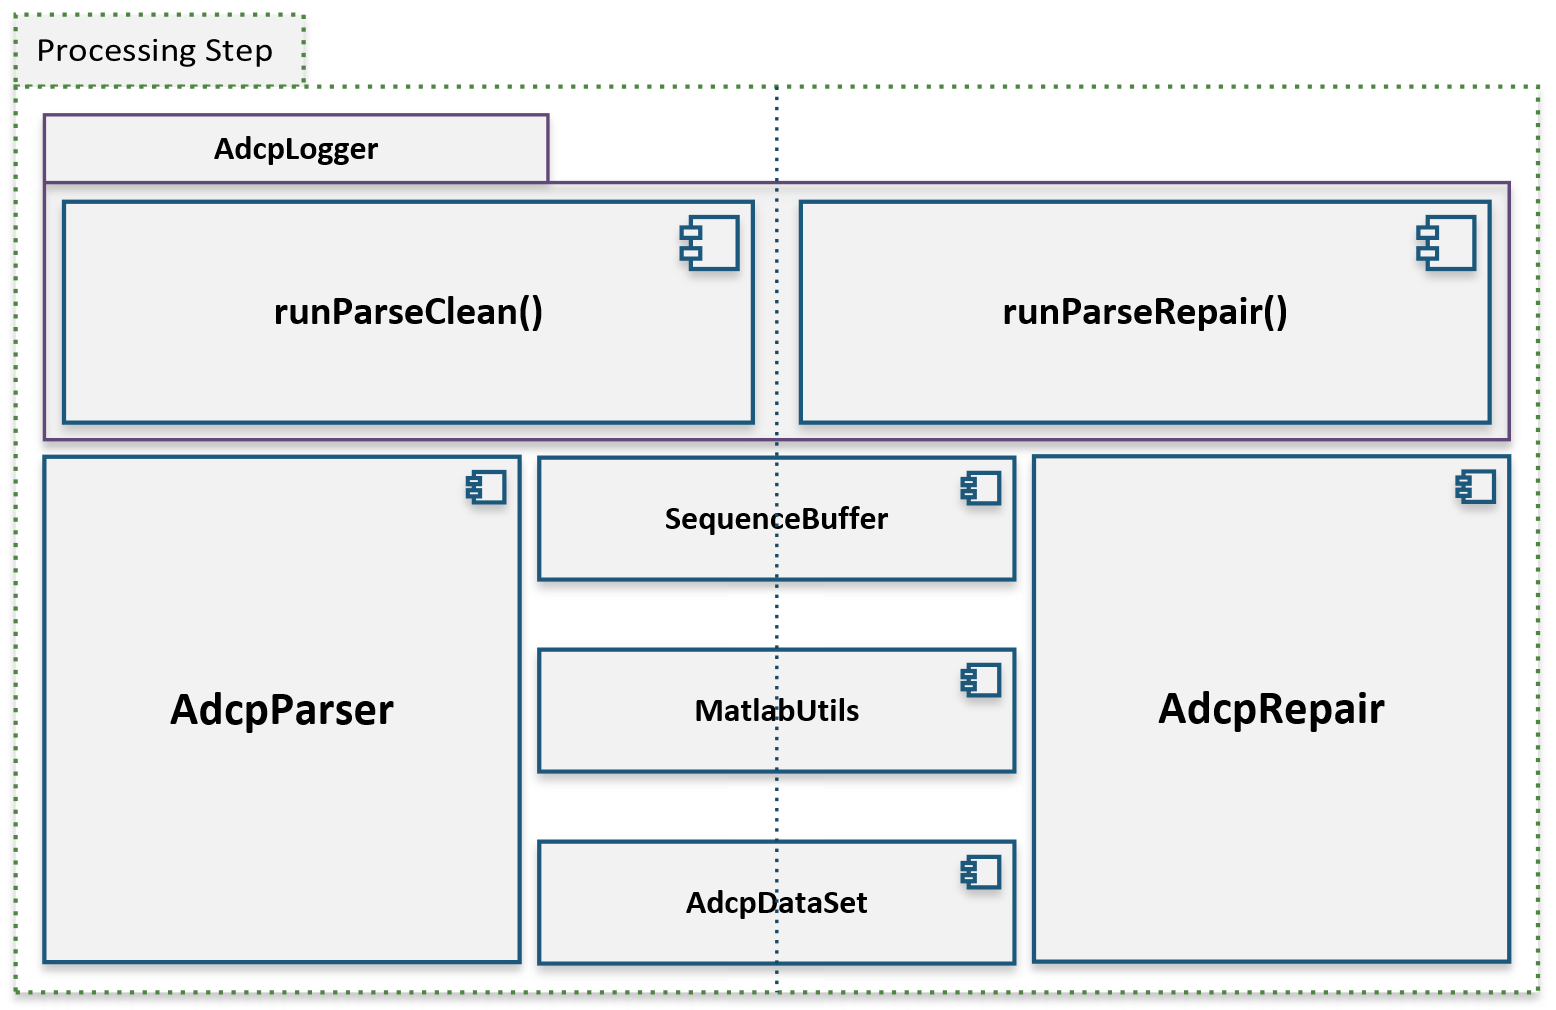
\includegraphics[width=0.8\textwidth]{components}
        \caption{A component diagram over all components used in the ADCP logger class.}
\end{figure}
A key part is the parser, a small state-machine used to extract complete ensembles from another component, the sequence buffer. The sequence buffer was introduced as buffer mechanism on top of an incoming data source. It should allow all-or-nothing reads on the host and be able to find specified sequences as the starting sequence of each ensemble described in the related work section. The decision to use such a buffer was for instance the aibility to decouple the ADCP parser component from the used input data source. It also moves the functionality of finding a sequence into the buffer and simplifies thus the components using this buffer. Another component is used for the Matlab related parsing of the ensembles.\\ In the developement process a request from General Acoustics e.K. regarding a current project in the Iraq where the repair of currupt ADCP data was needed, opened the path for an additional processing component. It was implemented also as a thread function in the ADCP logger class but uses a new parser class \texttt{AdcpRepair} again a state machine to collect the data from the sequence buffer. Such repair algorithms are very fragile and have to scope with a lot of error possibilities. The goal was to try a data recovery with a reasonable amount of effort. It was decided to correct one maby two byte errors in a matlab matrix, this reaults at around 10 allowed errors in one ensembles. A better recovery algorithm would need to make too much assumptions, and thus propably jeopardize dthe correctness of the data with false-correct values.\\
The output components for the output thread were again decided based on older use cases. Eighter binary file output for one result file, e.g. to merge a month of burst data files into one file, or binary file list output, to generate a list of files based eighter on timestamps or when no data arrives whilst on real time operation. The output components are message based, where a block of binary data is combined with a timestamp to a message. Thus it is possible to decouple the output from ADCP data structures and making it independant and usable for ather sensor types, as long as the output is binary.\\
Figure 3.3 shows all components of the decided architecture in a component diagramm the threads may be viewed also as components and are drawn as dashed components. The connecting FIFO data structures were left out to simplify the figure and get their attention later on.\\ 
\begin{figure}[h]
\centering
      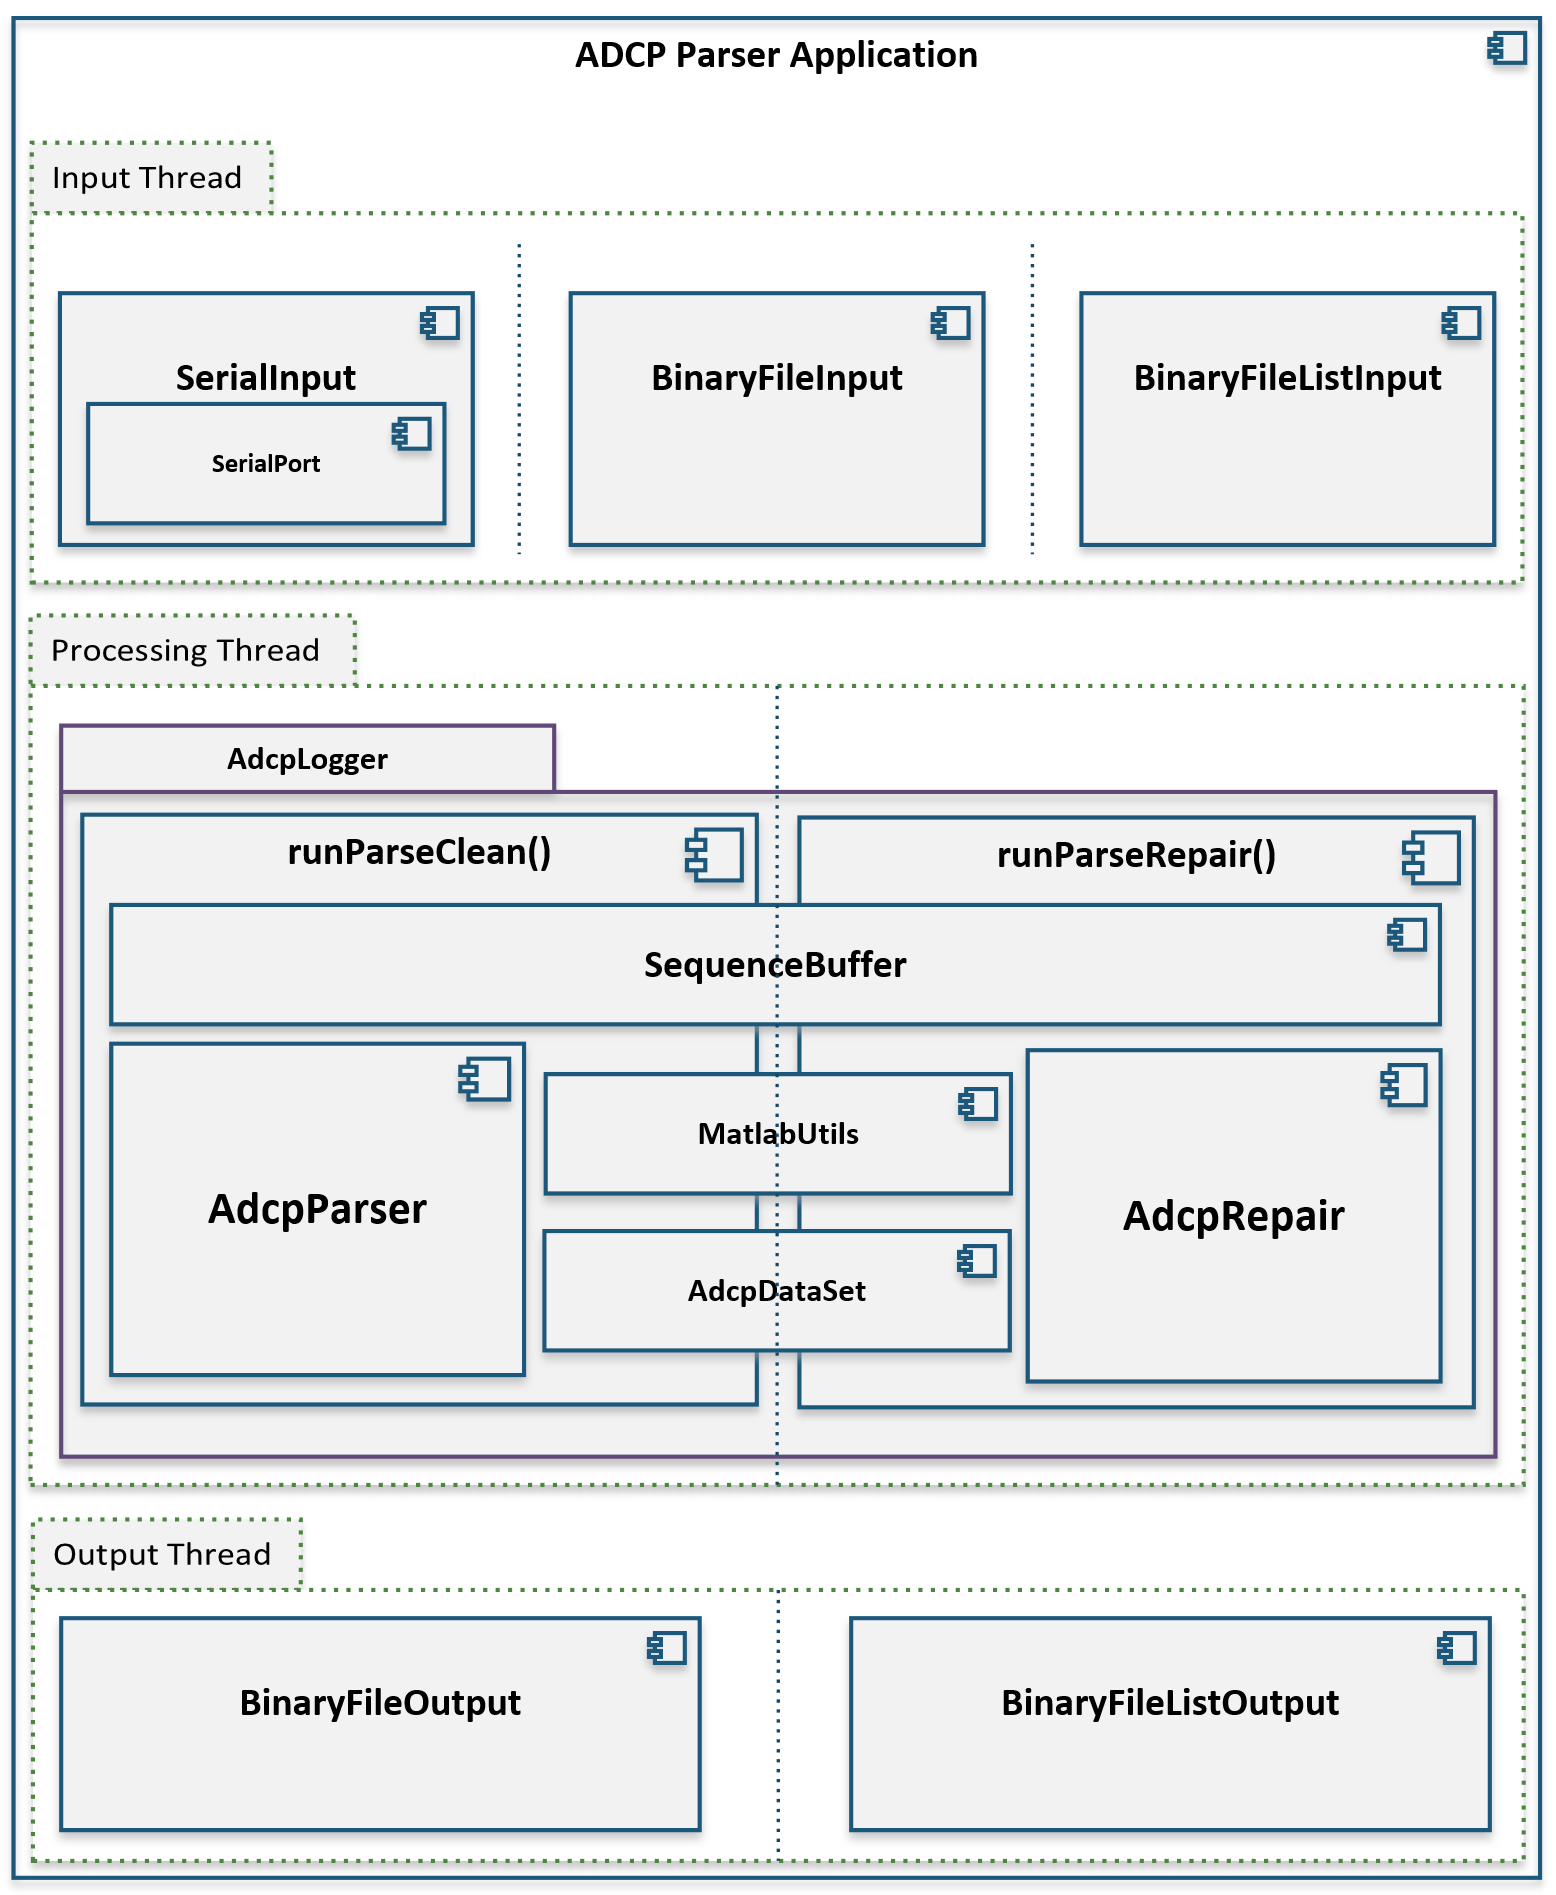
\includegraphics[width=0.8\textwidth]{all_components}
        \caption{A Component diagramm over all components used in the software}
\end{figure}
In reflection on the requirements the resulting architecture is structured, decoupled and formed around components. The Matlab component, the sequence buffer as well as the input-output components are completly indepent of the ADCP context and would be ready to use for other projects.

The design of the datastructures used in the application should also follow the guidlines formed by the requirements. 
\begin{figure}[h]
\centering
      \includegraphics[width=0.8\textwidth]{data structures}
        \caption{A class diagram representing the implemented data structures}
\end{figure}
Figure 3.4 shows an overview of the used classes. In this figure, a distinction of the modules was done by dashed rectangles. Only one data structure uses ineritance the ADCP ensemple with its matrice classes, in the other cases it was simply not neccessary! The degree of inheritance was tested in various scenarious from a complete flat hirarchie to the final version over three layers. The reason why inheritance was necessary in the first place, were the two different datatypes used in the ADCP data matrices. The decision for the current final approach resulted out of better usability in working with base class pointers. It saves a lot of code lines if one is able to iterate over an array of base class pointers instead of writing the code ten or more times. This way it is also possible to instantiate a \texttt{AdcpEnsemble} without preallocated matrice classes, and add them only if needed. There were arguments against this approach, especially performance wise because the downcasts were expensive, as the developement progressed it turned out that this was only a compiler setting. If the code was compiled for release, the compiler optimized as far as a concrete destinction between a high- or a low ineritance hierarchy was not detactable anymore.

\section{Implementations Specific Decisions}
For the developement process, some decisions had to be taken. Important was the choice of the developement environement. It was decided to develop on Windows and test the code on a small arm7 lowpower device. To be able to use the same compiler on both architectures it was needed to use another integrated developement environment (IDE) than the most famous C++ environement Visual Studio. The decision fell on CLion from JetBrains [] a relatively new IDE with alot functionality and identical usability than their allready well known Java IDE IntelliJ []. As compiler was GCC 4.9.2 chosen in conjuncture with MinGW 64 Bit from nuwen []. The reason were the allready integrated Boost libraries and the preinstalled CMake building tool.\\
The decision to work with the new C++11 instead of the old C++03 standard was quickly taken. It introduces a lot new functionality, some of it crucial for efficiency (\texttt{std::move}), memory management (\texttt{std::shared\_ptr}) and threading (\texttt{std::atomic}). During the implementation period in early 2016 C++11 was allready widespread and compatible compilers available in almost every platform. On the target platforms for the software, even C++14 was allready available.
\subsection{Library Decisions}
This sections will shortly describe the choices that were made in the selection of used libraries. It highlights only the reasons of the choice, the used libraries were allready described in Chapter 2.

The first library introduced was Boost. When working with C++ and a portability requirement, one of the first libraries used is Boost. Boost is a collection of portable C++ source libraries covering a broad spectrum off applications. The libraries provide reference implementations that may be later included in the C++ standard. A large part of boost was allready included in the new C++11 Standard [] but not everything needed in this project. The decision to use Boost was quickly taken, mainly because the compiler in MingGW did not support the standardized \texttt{std::thread} which was introduced in C++11 and thus leaving no other choice than Boost for portable threading. Otherwise the Asio library for network communication was also a driver to use Boost, it was used for the portable communication over serial ports. The used version of Boost was at the time the newest (v 1.60.0) it was the first one where a lot of code was implemented in C++11 allowing e.g. the use of efficient move semantics.\\
With the inclusion of Boost the decision on other libraries was driven by its availability in Boost. It would make no sense to introduce other dependencies into the project if a solution was available in boost. The following choices libraries were influenced mostly by on their availability: Boost Program Options, used to parse program parameters from a INI file. This library was the only viable option, it was able to combine parameters from the commandline as well as from a configuration file. Other options like getop [] or a beatiful small library TCLAP [] were only focussed on the commandline arguments. The other library where the decision was heavily influenced by the use of Boost, is the test framework Boost Test []. The Clion IDE offered the integertion of Google's testing framework gtest [] which would have offered a comfortable interface with grafical response on the test results. Problems with the MinGW platform as well as the drawback of an additional dependency drove the decision towards the allready integrated Boost Test.

In the developement process, two external components were included. The first one was a lockfree thread-safe concurrent queue developed by Cameron Desrochers []. He developed a Multi-Producer-Multi-Consumer (MPMC) queue with one of the fastest implementations e.g. compared to Boosts lockfree datastructures. This queue was used as connection between the threads, and using explicit consumer- and producer tokens the queue was used as a Singel-Producer-Singel-Consumer (SPSC) queue. In the decisions which technology should be used to connect the threads the first consideration was the use of the C++ Standard Library (STL)  input and output streams. The lack of threadsafety of most STL data structures and streams would have made this approach complicated as the synchronization of the threads would have been done by hand. The queue developed by Cameron was the best choice to connect the threads and removed the need of manual thread management, it outperformed e.g. the boost lockfree queue [http://joshitech.blogspot.ch/2015/02/queue-benchmark.html].\\
The second external code used, is just a beatiful implemented wrapper around the serial port class of Boost Asio and was implemented by Terraneo Federico []. The reason to use this class was only a simplification of the developement process which allowed to set the focus on other parts of the project implementation.

For the sake of simplicity the following namingscheme for files with ADCP data was decided. The file extension is a point followd by three letters. Left of the extension follows a  eight-digit number which is again followed on the left side by a unspecified prefix.

$$ \underbrace{ADCP}_{\text{Prefix of variable length}}\underbrace{00000123}_{\text{Eight-digit number}}\underbrace{.bin}_{\text{Extension}}$$

%-------------------------------
%-------------------------------
%-------------------------------
\chapter{Implementation}
This chapter gives a detailed insights on implementation specific aspects of the project. In the first three sections, the standalone components without ADCP related depencencies  are introduced, followd by a descrition of the parser class. The last section puts the components together and describes the architecture of the main program.  
\section{Matlab Component}
Section 2.2 in Related Work describes the data generated by an ADCP. It was shown that the payload of each ensemble is serialized in a Matlab version 4 file format. This format is used by General Acoustics e.K. for other sensor types e.g. a sub-bottom profiler. The high propability to reuse the code and algorithms related to the Matlab v.4 format predestines for a clean, independant and selfcontained code. To ensure the required independency the Matlab component was implemented and tested before the other components and the main program.\\
The implementation strongly followed the official Matlab v4. file structure documentation []. The structure defined there has a lot more possible data types and matrice types than used by the ADCP. As example, in a Matlab v.4 matix the data may be stored as a sparse matrix, but this feature is not used for ADCP ensembles. The unused features were prepared but not implemented as seen in figure 4.1.
% prepared code snippet
\begin{figure}[h]
\centering
      \includegraphics[width=0.8\textwidth]{unimpl}
        \caption{Code snippet of not implemented logic.}
\end{figure}
The decision to skip the implementataion of project unrelated parts helped to focus the programming efforts on other more complex parts of the project. The library is well structured and easily extendable, thus it will be a simple task to extend it if asked in forthcoming projects.
% matlab structure
\begin{figure}[h]
\centering
      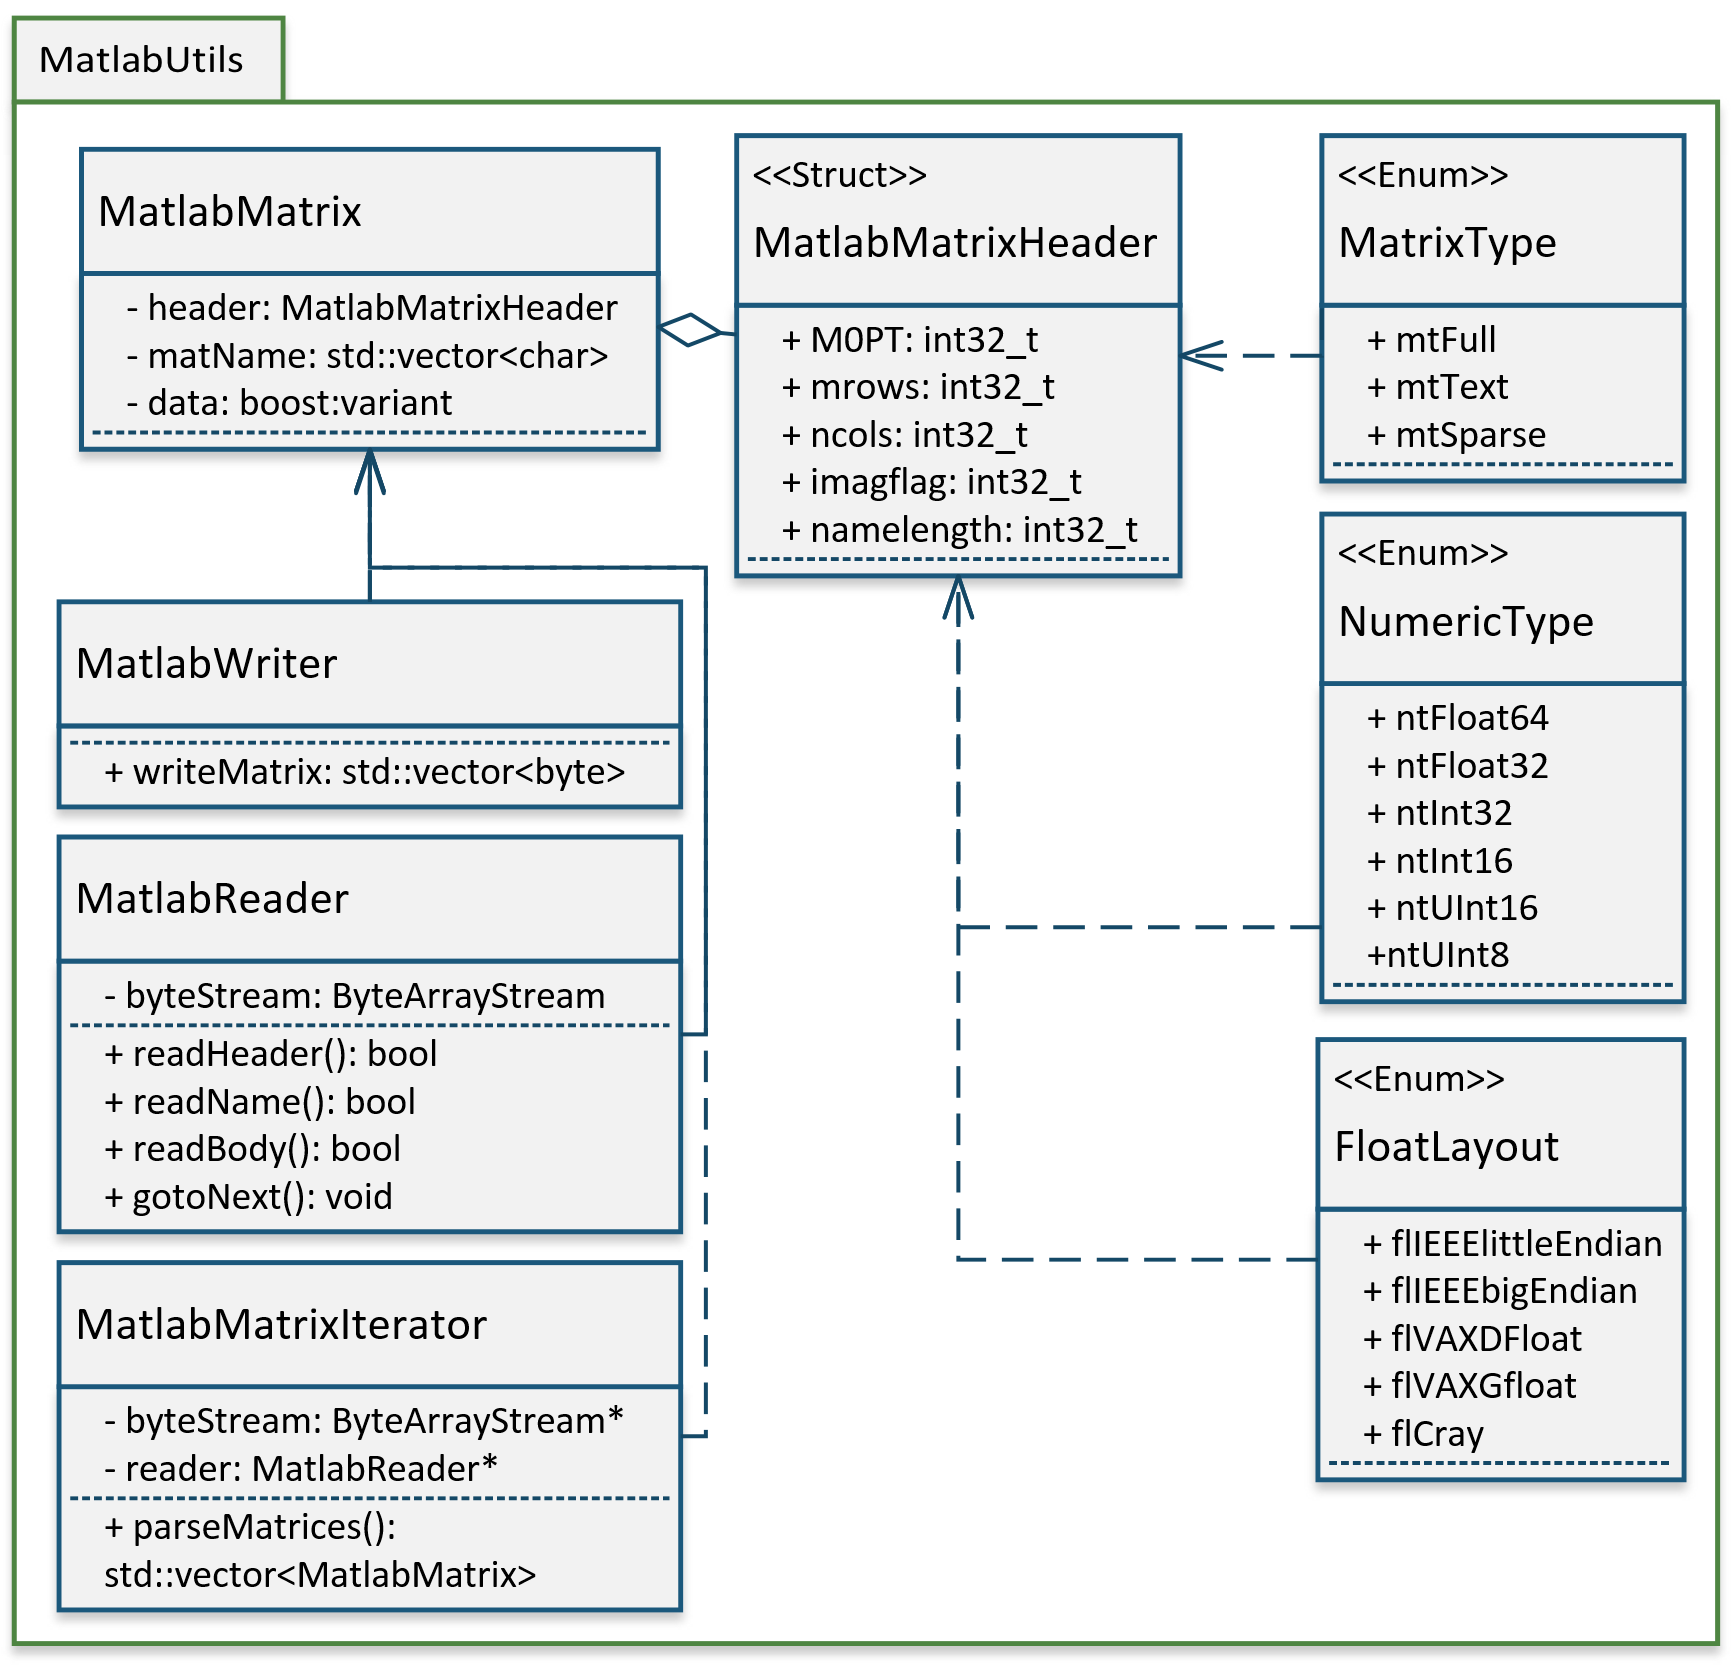
\includegraphics[width=0.8\textwidth]{mlab}
        \caption{A class diagram as overview over the matlab component.}
\end{figure}
The structure of the component is presented in Figure 4.2. The \texttt{MatUtils::MatlabMatrix} is the core class of the Matlab component and stores a matlab matrix, the other classes are used to serialize and deserialize these matrices. The \texttt{MatlabMatrix} class is described in the next subsection.
\subsection{Matlab Matrix Datastructure}
As presented in figure 3.6 a matlab matrix contains a \texttt{MatUtils::MatlabMatrixHeader}. The header contains five \texttt{uint32} Integers specifiying the rest of the Matrix and is implemented as a struct. The first integer, also called \texttt{M0PT}, is composed out of three other integers. The value is calculated as follows:
$$M\cdot1000 + 0 \cdot 100 + P\cdot 10 + T$$
M represets the float layout which specifies how the float is stored in bytes. Only little and big endian were considered for this project. P is the numerical type of the matrix content and T is the matrixtype which holds if the matrix is eighter a full matrix, sparse matrix or a matrix containing text. All three values are implemented as enums, their implementation is shown in figure 4.3.
\begin{figure}[h]
\centering
      \includegraphics[width=0.8\textwidth]{mlab_struct}
        \caption{A code snippet showing the used enums and structs in the Matlab header.}
\end{figure}
The next two integers in the header contain the number of rows and columns. Next follows a flag if the matrix has an imaginary part, which would double the amount of data used. The last integer of the Header contains the number of characters from the matrix name incremented by one to account for the string termination character.
The \texttt{MatlabMatrix} class additionaly contains a vector of \texttt{char}'s to store the matrixname.\\
The matrix data is stored in a templated \texttt{boost::variant} vector to allow a range of data types for the data. The fairly complicated templating (figure 4.4) needed to achieve this goal was taken from  a great answer at Stackoverflow [], this way the otherwise needed inheritance hierarchy was bypassed. 
\begin{figure}[h]
\centering
      \includegraphics[width=0.8\textwidth]{mlab_templ}
        \caption{A code snippet showing the templating to allow various types in a Boost variant.}
\end{figure}
%-------------------------------
%-------------------------------
\section{Sequence Buffer}
The idea of the sequence buffer has its origin at General Acoustics e.K. It serves as a buffer between binary input streams or input queues and a consumer. The buffer can be used if the \texttt{read()} operations should be done in a all-or-nothing way. The buffer has a \texttt{find()} method that searches for a sequence in the current buffer.\\
The buffer has three properties that define how the buffer mechanism works. The buffer can be \texttt{hungry}, with this property on each \texttt{load()} operation it will load the maximal number of bytes that can be filled into the buffer. If the second property \texttt{angry} is \texttt{true} the buffer throws an exception when the \texttt{find()} method fails and the buffer is full. The third option \texttt{autodiscard} states if, in case of a  \texttt{find()} failure the buffer should drop bytes to prevent a deadlock.\\
The set combination of these properties in conjunction with the preset buffer size should be considered carefully. If the byte sequence which should be found, is longer than the maximal buffersize the \texttt{find()} method will allways report \texttt{false} and the application ends in a deadlock. The same thing can happen if the buffer is neighter \texttt{angry} nor on \texttt{autodiscard}. In these cases the application has to prevent the deadlock.\\
The maximum buffer size is set at instantiation, but extends itself based on the size of the requested \texttt{read()} and thus make sure that the buffer has enough space for a read.\\
The implementation was done specifically for the moodycamel concurrent queue. Other sources can easily be added for different projects. The buffer could also be extended to support \texttt{readline()} operations on \texttt{CRLF} delimitered data. The stubs are allready prepared.\\
Figure 4.5 presents the simple API as a class diagram:

\begin{figure}[h]
\centering
      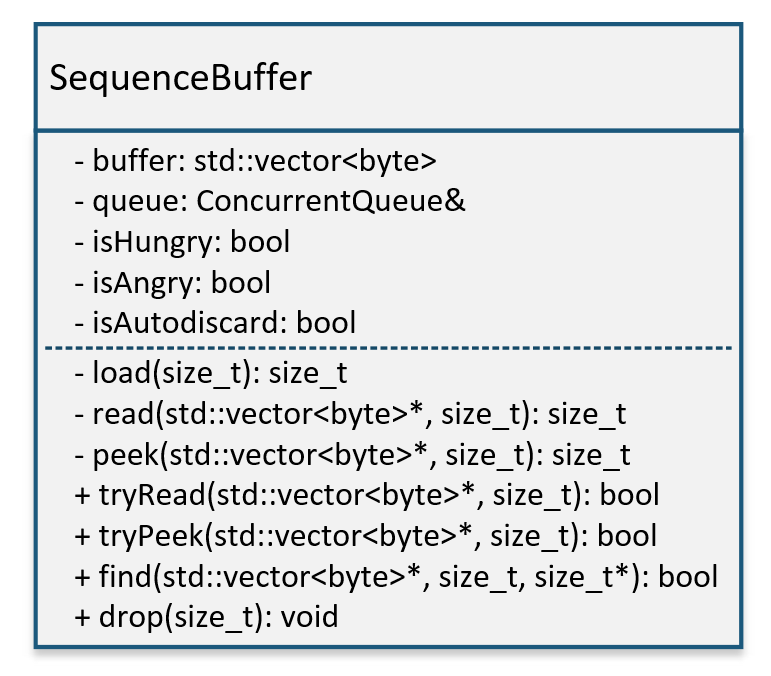
\includegraphics[width=0.8\textwidth]{seqbuf}
        \caption{A class diagramm of the sequence buffer.}
\end{figure}

%-------------------------------
%-------------------------------
\section{ADCP Logger}
The heart of this software project was the implementation of the ADCP logger application. It integrates the seperately developed components and forms the main program. This section shows the result of the implementation, explaining the architecture and specific technical specialyties in a detailed top down approach.\\
As specified in the design decisions, the architecture was implemented in a piplined input-processing-output way. The program allows the execution of different components for each pipeline step. A configuration file is used to tell the program which component should be instantiated. The Boost Program Options library was used to parse the configuration file and set all required parameters, Figure 4.1 shows an example of a configuration file. It conveniently allows to check for invalid parameters and produces nicely formatted help output.

\begin{figure}[h]
\centering
      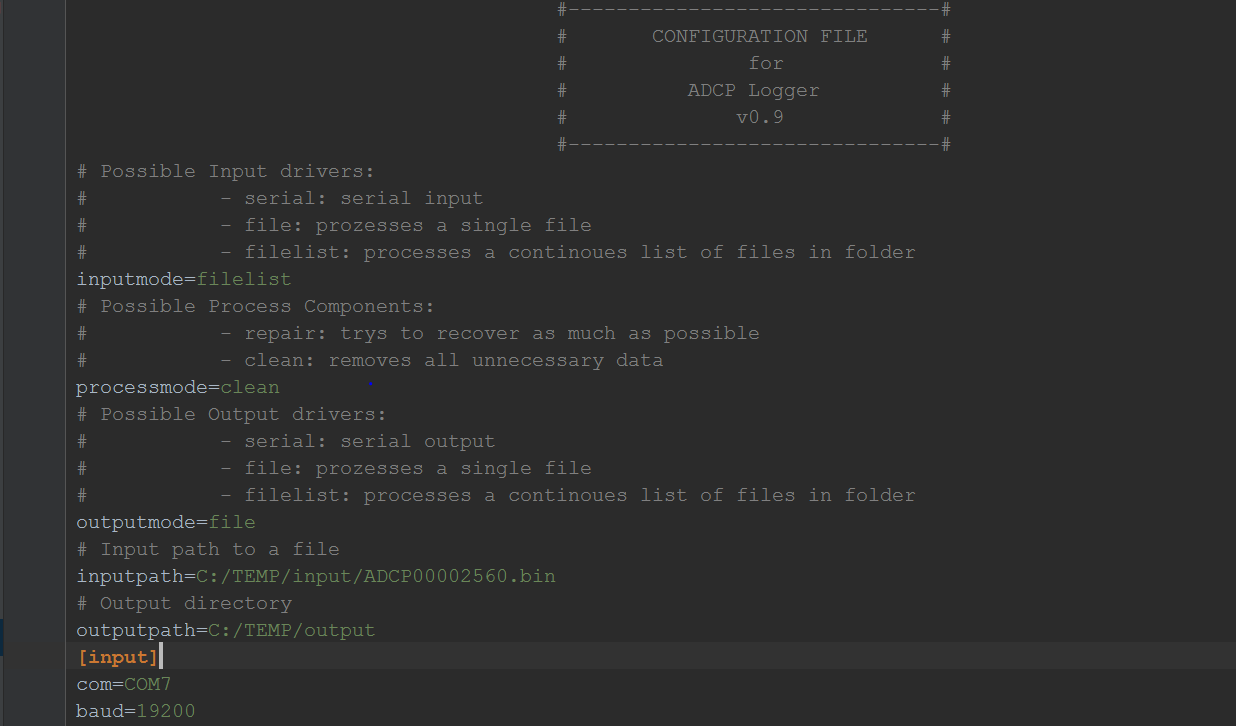
\includegraphics[width=0.7\textwidth]{config}
        \caption{A Snippet of a configuration file for the ADCP logger application}
\end{figure}

Each pipeline step is implemented as a thread. Figure 4.2 shows a dataflow model where the circles represent the threads. 

\begin{figure}[h]
\centering
      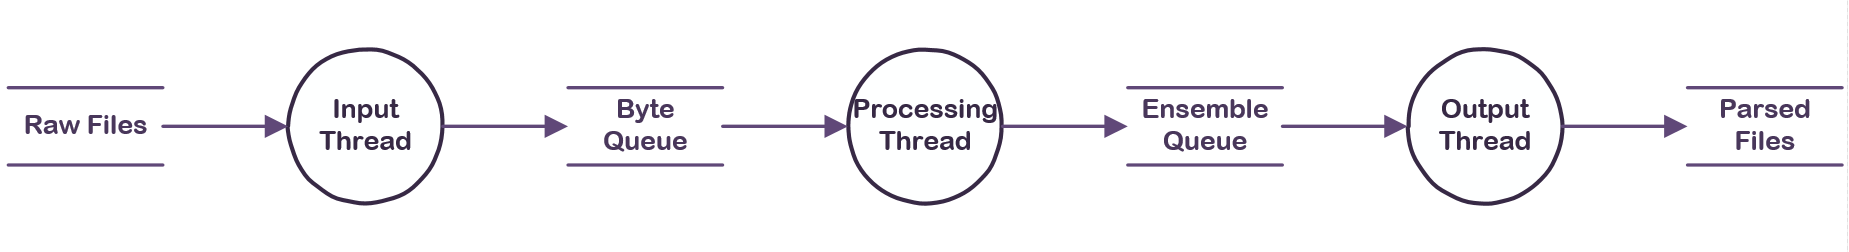
\includegraphics[width=0.95\textwidth]{dfd}
        \caption{A high-level Data-Flow-Diagram }
\end{figure}

 All threads are connected over moodycamels lockfree concurrent queues [], in the figure represented as data store objects. The queues are set up as Single-Producer-Single-Consumer (SPSC) queues and use explicit producer and consumer tokens to maximise performance. Figure 4.3 shows how the token is used to dequeue elements from an input queue.

\begin{figure}[h]	
\centering
      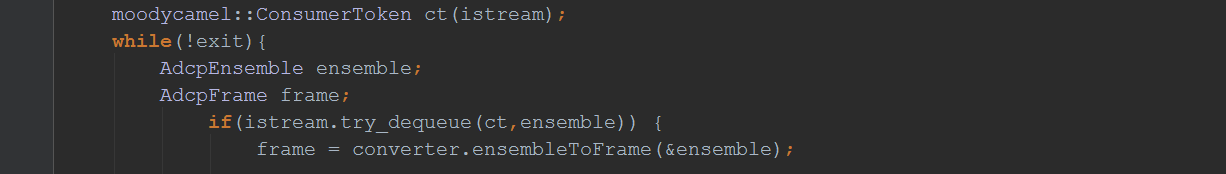
\includegraphics[width=0.95\textwidth]{ct}
        \caption{Codesnippet showing the use of consumer tokens}
\end{figure}

The threads run concurrently until the end of the execution. Each thread exits if its predecessor is finished. If this is the case, the thread synchronises with its predecessor over an atomic boolean value. It is important that the memory state of the predecessor gets propagated to the thread recieving the exit signal. The implementation of the memory propagation was done with the new C++11 \texttt{std::atomic\char`_thread\char`_fence} memory barriers. This step was needed that the thread determined to exit, can reliably see if it's input queue is empty. The critical function here is the \texttt{moodycamel::size\char`_approx()} function. It only returns the correct size of the queue if the memory effects of the enqueue operations in the predecessor threads have propagated. With the use of the described memory fences this state can be reliably provided. How this was implemented is shown in figure 4.4

\begin{figure}[h]
\centering
      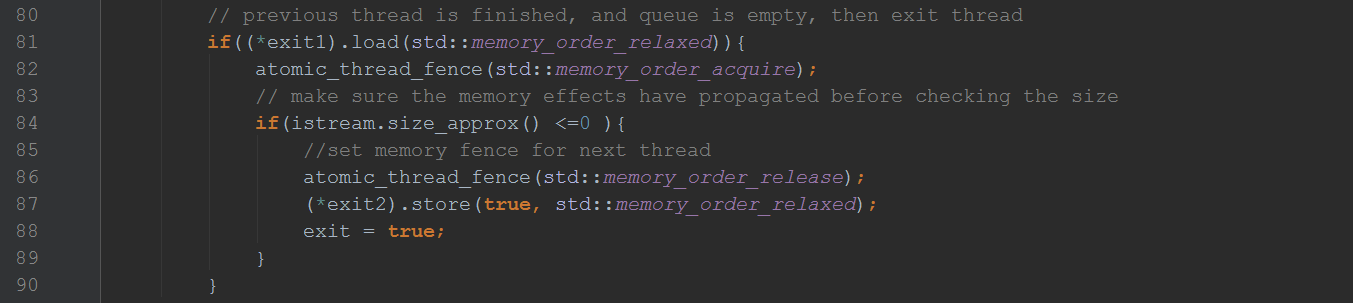
\includegraphics[width=0.95\textwidth]{memory_barrier}
        \caption{Codesnippet highlighting the memory barriers}
\end{figure}

This architecture would allow to insert eighter more components to select at each step or extend the model with a reasonable number of new steps e.g. a second processing step. The system of component selection and thread termination stays the same.\\
The next three sections look at the currently implemented steps of the processing pipeline. A class diagramm is presented for each step. The diagrams omit getter and setter methods as well as constructors to simplify the diagramm. If a component was allready shown before, it is only added as a simplified package to save space.
\subsection{Input Step}
In Chapter 3 an overview of the input components was described. The following class diagramm (figure 4.5) shows the three input components \texttt{SerialInput}, \texttt{BinaryFileInput} and \texttt{BinaryFileListInput}. All three classes are derived from the abstract class \texttt{BinaryInput}. The classes are located in the file \texttt{BinaryIO.h} together with the output classes.

\begin{figure}[h]
\centering
      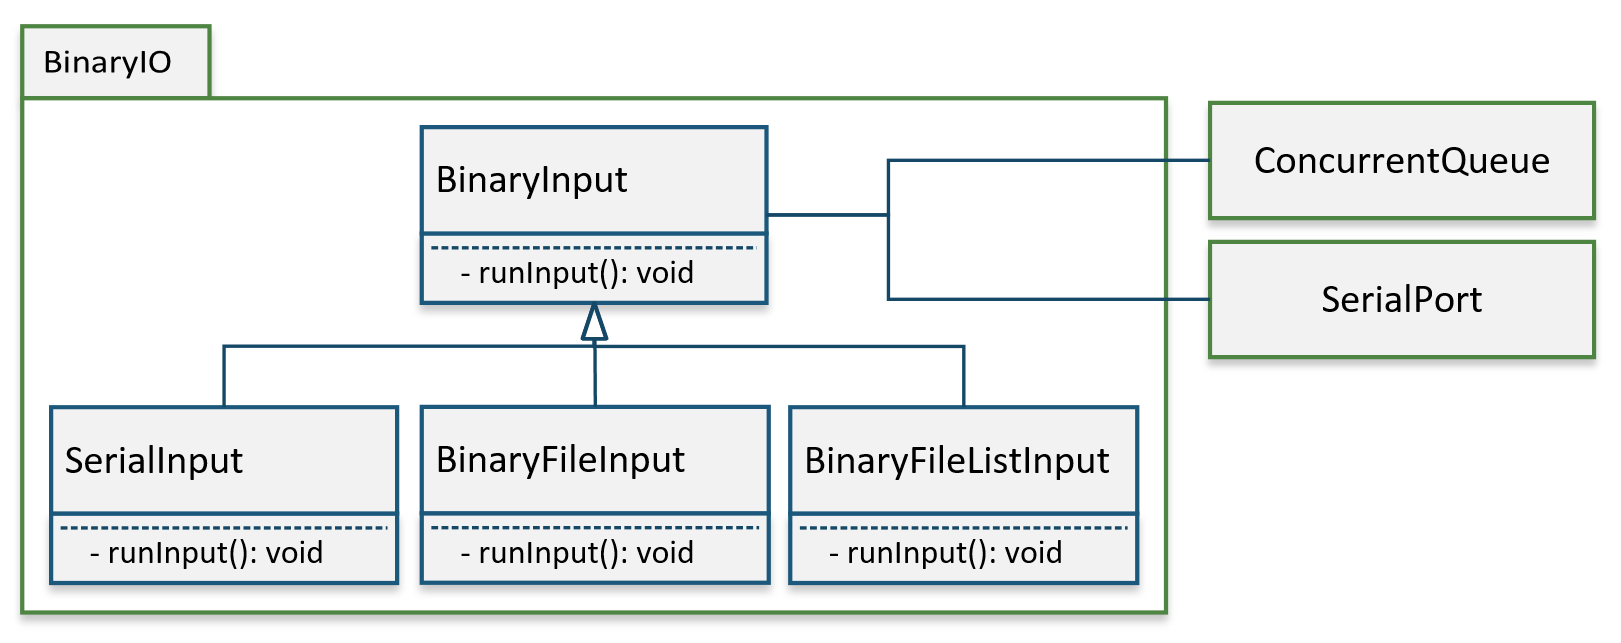
\includegraphics[width=0.95\textwidth]{input}
        \caption{A class diagramm of the input components}
\end{figure}

The classes have only the \texttt{runInput()} method where the business logic of the component was implemented. One of these functions will be executed by the input thread. \\ The \texttt{SerialInput} class simply polls a serial port regularly and tries to enqueue the data to the queue, if it is not able to enqueue, it buffers the data in a vector and tries it again in the next loop. If the buffer exceeds its maximum size, old data is thrown away. With proper parametrization of the queue- and buffersizes depending on the host machine this should never be the case!\\
The \texttt{BinaryFileInput} class is used to process one file. It first checks the availability of the file and calculates the filesize as nubmer of bytes. Depending on that size, eighter the whole file is enqueued at once, or it is enqueued in chunks. Once again one has to be careful to set the parameters correctly or else the application ends up  in a deadlock.\\
The \texttt{BinaryFileListInput} class does essentially the same thing than the \texttt{BinaryFileInput} but iterates over a directory and processes all files that follow the naming scheme defined in section 3.3 and have a number bigger than the startingfile.
\subsection{Processing Step}
The processing step contains most of the business logic implemented in this project. Figure 4.10 presents the class structure used for this step. The Matlab component as well as the sequence buffer were presented in section 4.1 and 4.2 and are only included as packets.

\begin{figure}[h]
\centering
      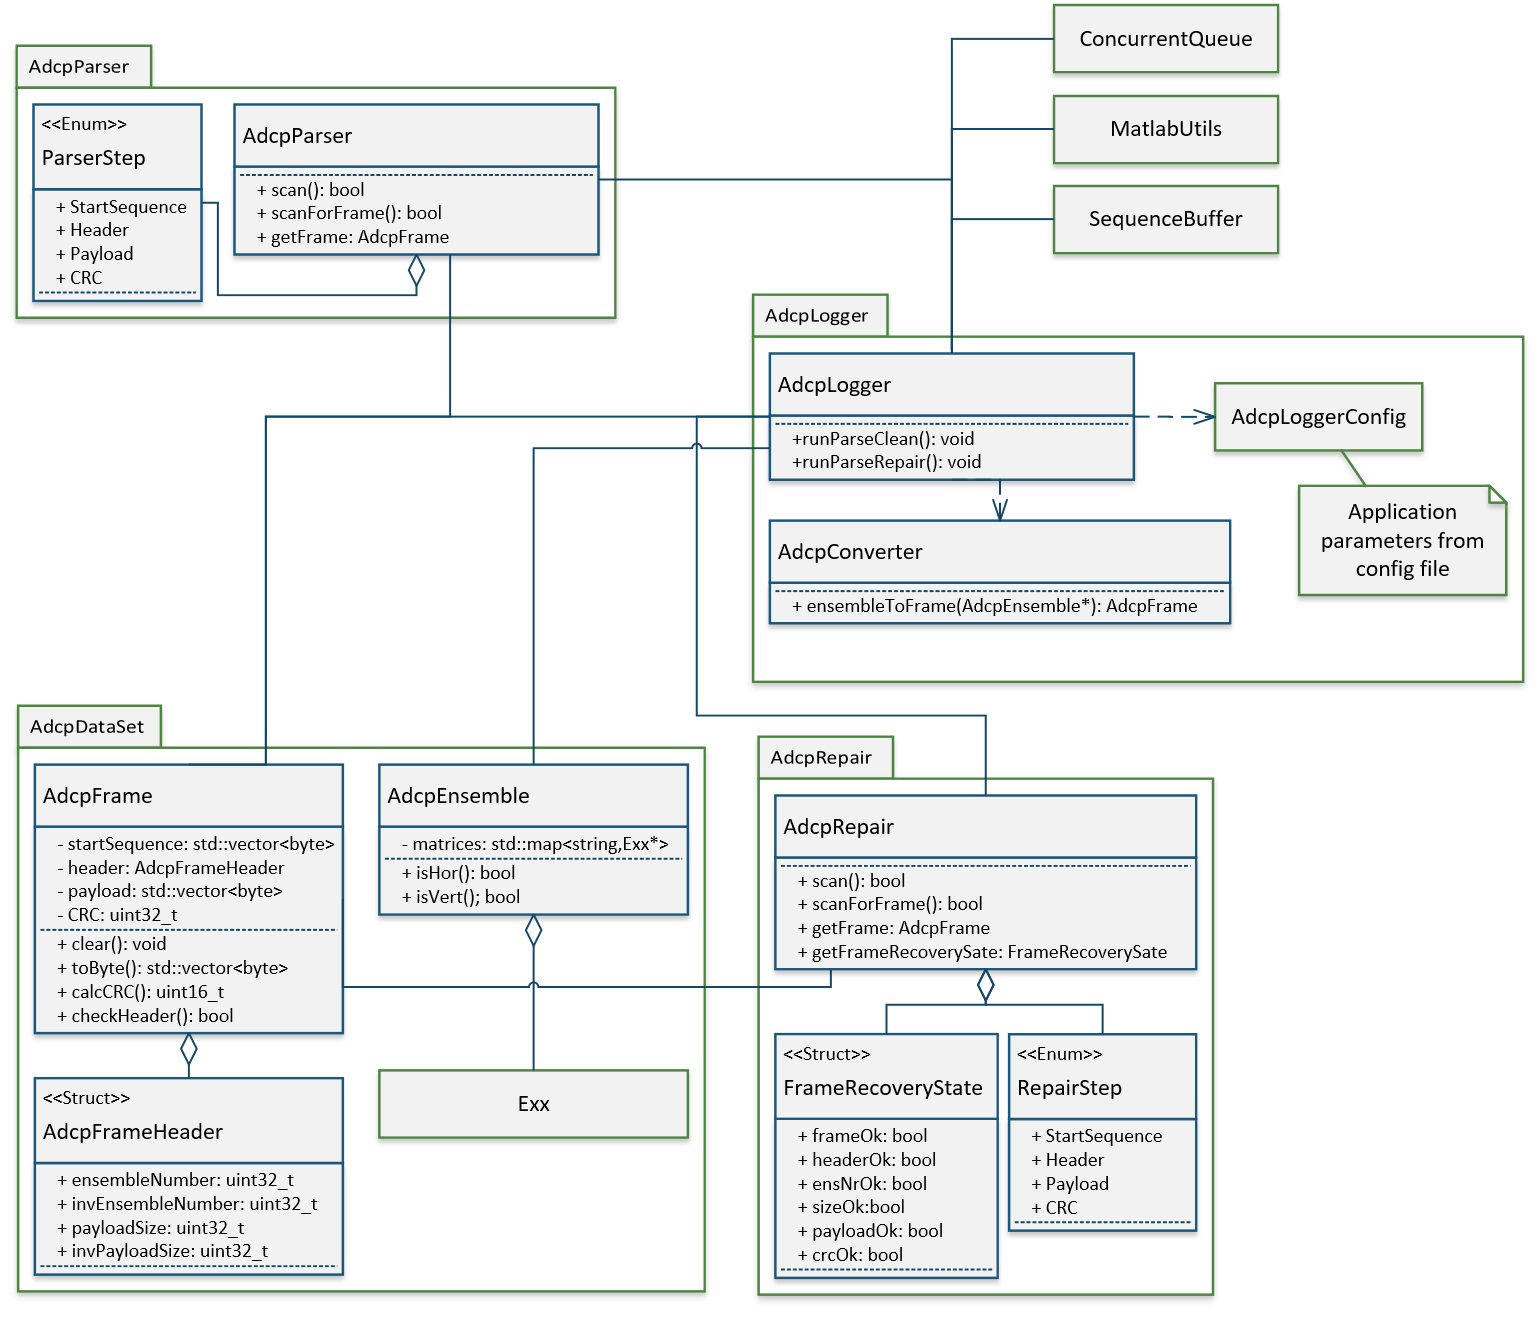
\includegraphics[width=0.95\textwidth]{logger_class}
        \caption{A class diagramm of the components used for the processing step}
\end{figure}

In the center is the \texttt{AdcpLogger} class. It has two methods \texttt{runParseClean()} and \texttt{runParseRepair()}. These two methods can be seen as the two processing components shown in the component overview in section 3.3. One of them gets executed in the processing thread.\\
The \texttt{runParseClean()} method satisfies the requirement to parse the incoming ADCP data and throw away the unused parts. It uses the \texttt{SequenceBuffer} class to buffer the incoming binary data from the input queue. The \texttt{AdcpParser} class is then used to extract complete \texttt{AdcpFrames} from the buffer.\\
The parser itself is a small finite state machine shown in figure 4.11. It is divided into four states. If the parser enters a new state, the code belonging to this step is executed, depending on the result it can enter into a new state or has to run the state code again in the next iteration. The fist state is \texttt{StartSequence}. In this state the parser uses the \texttt{find()} function of the sequence buffer to find the ADCP start sequence in the input queue. If successful, the parser transitions to the secend state \texttt{Header} and reads the ADCP header. If the header is invalid the frame will be discarded and the parser is reset to the \texttt{StartSequence}. When a correct header is found the parser jumps to state three \texttt{Payload} and reads the number of bytes specified in the header into the frame payload. In this step the parser transitions always to the last state \texttt{CRC} where it reads the target CRC value from the stream and compares it to the actual CRC calculated from the previously read payload. Depending on the result the frame is eighter trown away when the CRC's are not equal, or it is made available for collection. If in eighter one of the stats the sequencebuffer can't deliver because its queue is empty, the parser stays in the same state.

\begin{figure}[h]
\centering
      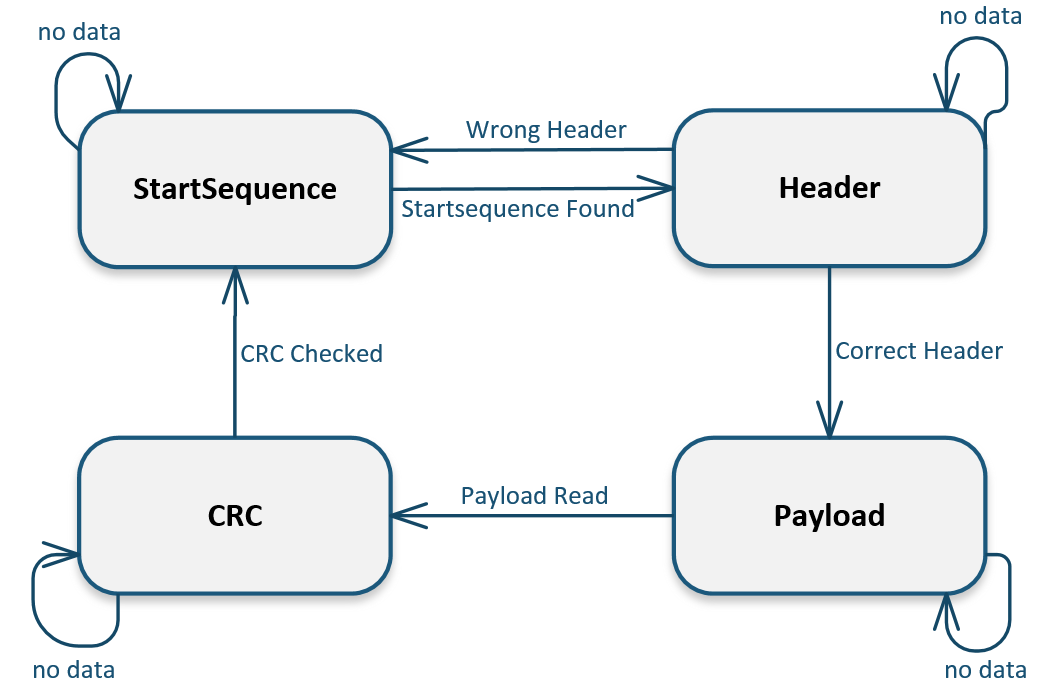
\includegraphics[width=0.95\textwidth]{parser}
        \caption{A state diagram of the ADCP parser}
\end{figure}

With this behaviour of the parser the \texttt{runParseClean()} method is  guaranteed to get always complete frames. The payload of these frames is then processed with help from the \texttt{MatlabUtils} component to extract the Matlab matrices which then are filled into an ensemble. At this step the cleaning happens. The ensemble is only filled with matrices needed for the further processing by General Acoustics e.K. At the moment the matrices E000001 or E000003 and E000008, E000009, E000015 are kept.\\
The ensembles are then converted back to a ADCP frame and then into a byte sequence. The byte sequence is then packed into a binary output message together with the timestamp from the ensemble. The Message is then enqueued to the output queue, available for the output step.\\

The \texttt{runParseRepair()} component was introduced as a result from an urgent request from General Acoustics. It was needed to repair and save as much ADCP data as possible from a corrupted stream. The problem was a defective communication between an ADCP and the data logger. The data stream lost bytes fairly regurly.
The task turned out to be much more complicated than thought at first. A lot of assumptions had to be taken, e.g. only frames with a complete start sequence were considered. Another preset constraint was the number of bytes that were allowed to miss in each matrix. The result of considering various error scenarios was a new parser class, th \texttt{AdcpRepair}. It is also a state machine but is able to extract also ensembles containing errors. The data to be extracted has to be at least more or less recognizable as a ADCP frame to be able to reconstruct it. Figure 4.12 shows the state machine of this parser.\\

\begin{figure}[h]
\centering
      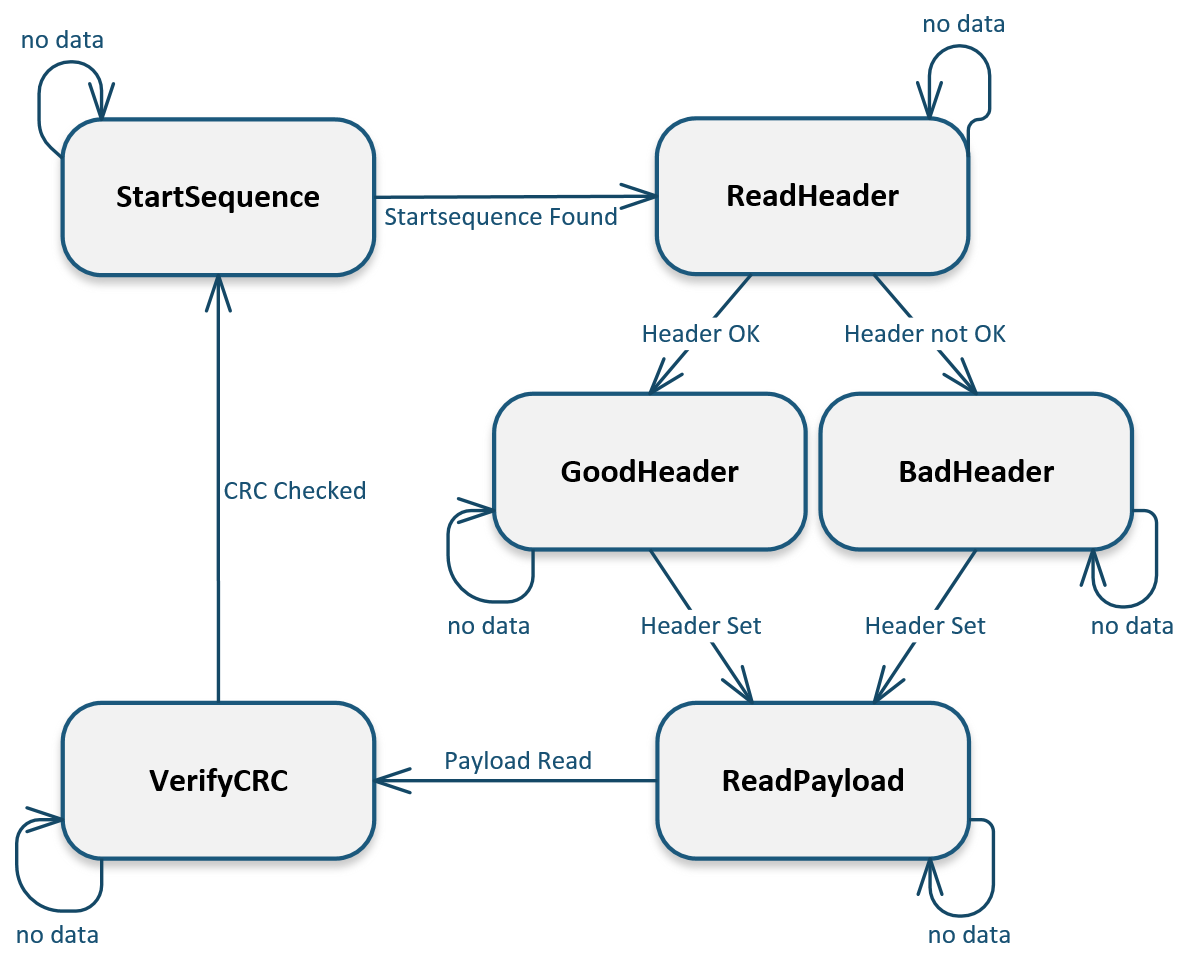
\includegraphics[width=0.95\textwidth]{repair}
        \caption{A state diagram of the ADCP repair parser}
\end{figure}

In the \texttt{runParseRepair()} method the recieved frames are processed in the hope to recover as much as possible. Propably the most important correction happens at the moment where the byte stream is converted to ints or floats. If a byte is missing the generated number is semantically wrong or even not considered as a number. Figure 4.3 shows the code snippet that tries to find where the byte is missing, and searches for the next possible healty value.\\
After recovering as much as possible, all data like the timestamp or the ensemble number are tested again for plausibility, if everithing seems fine the frame is converted to a message and enqueued reade for the output thread.
\begin{figure}[h]
\centering
      \includegraphics[width=0.95\textwidth]{repair_byte}
        \caption{Code snippet from the repair function, it finds missing bytes}
\end{figure}
This Algorithm only works reliable if the number of missing bytes is not too low. It also has room of improovement but it was not a core requirement of this project, so further developement would have meant unnecessary effort. The result can be seen as `good-enough'. Originally only 20 out of 2048 ensembles were healty, with this function the number could be raised to over 800 which was enough for further wave analysis.

\subsection{Output Step}
The output step 

%-------------------------------
%\chapter{Testing}


 